\documentclass{beamer}
\usepackage[utf8]{inputenc}
\usepackage[bahasa]{babel}
\title{Membuat Presentasi Dengan Latex Beamer}
\author{@btatmaja}
\date{\today}
\begin{document}
	\frame{\titlepage}
	\frame{
		\frametitle{Table of Contents}
		\tableofcontents
	}
	
\section {1. Membuat list}
\begin{frame}[t, fragile]{Slide pertama}
Berikut adalah list berupa bullet:
\begin{itemize}
\item List1
\item List2
\item List3
\end{itemize}
\end{frame}


\begin{frame}[t, fragile]{Slide kedua}
Berikut adalah list berupa angka:
\begin{enumerate}
\item List1
\item List2
\item List3
\end{enumerate}
\end{frame}

\section{2. Memasukkan gambar}
\begin{frame}[t, fragile]{Slide berisi gambar}
%\includegraphics[width=4in]{pict/gedit-symbol.png}
\end{frame}

\section{3. Membuat kolom}
\begin{frame}[t, fragile] {Membuat kolom}
Ada kalanya anda perlu membuat kolom, misalnya, gambar dikiri dan teks dikanan, contohnya seperti dibawah ini \\
\begin{columns}
\column{.5\textwidth}
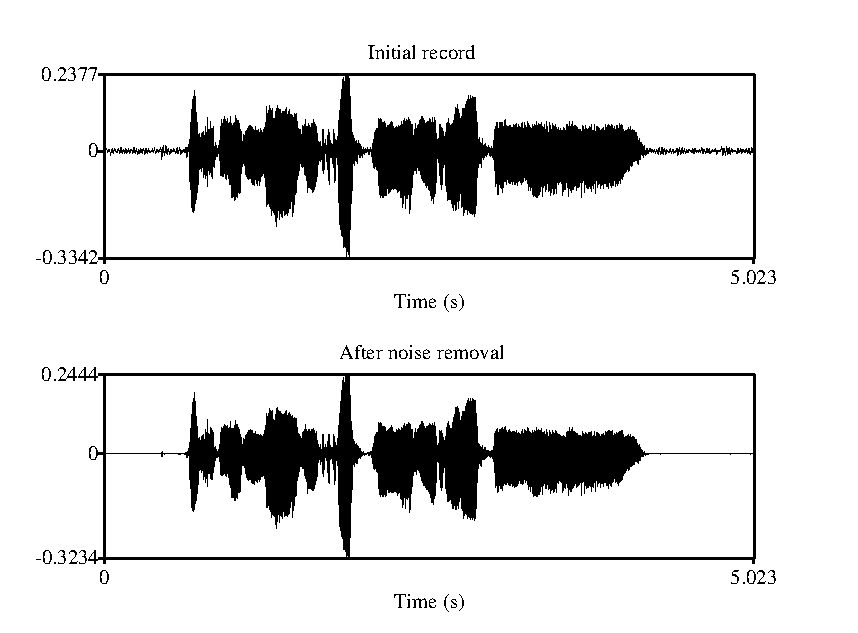
\includegraphics[width=2in]{pict/praat.eps}
\column{.5\textwidth}
\begin{verbatim}
\begin{columns}
\column{.5\textwidth}
% isi kolom
\column{.5\textwidth}
\begin{verbatim}
\end{verbatim}
\end{columns}
\end{frame}

\end{document}
